% A Beamer template for Central China Normal University 

\documentclass[aspectratio=169]{beamer}
\usepackage{ctex, hyperref}
\usepackage[T1]{fontenc}

% other packages
\usepackage{latexsym,amsmath,xcolor,multicol,booktabs,calligra}
\usepackage{graphicx,pstricks,listings,stackengine,subcaption}
\usepackage{CCNU}


\usefonttheme{serif}

\author{韩子坚}
\title{组会分享}    %标题
\subtitle{Case-Based or Rule-Based: How Do Transformers Do the Math? \\ Qwen2.5-Math Technical Report: Toward Mathematical Expert Model via Self-Improvement}    %副标题
\institute{华中师范大学计算机学院}    %机构
\date{\today}     %时间


% defs
\def\cmd#1{\texttt{\color{red}\footnotesize $\backslash$#1}}
\def\env#1{\texttt{\color{blue}\footnotesize #1}}
\definecolor{deepblue}{rgb}{0,0,0.5}
\definecolor{deepred}{rgb}{0.6,0,0}
\definecolor{deepgreen}{rgb}{0,0.5,0}
\definecolor{halfgray}{gray}{0.55}

\lstset{
    basicstyle=\ttfamily\small,
    keywordstyle=\bfseries\color{deepblue},
    emphstyle=\ttfamily\color{deepred},    % Custom highlighting style
    stringstyle=\color{deepgreen},
    numbers=left,
    numberstyle=\small\color{halfgray},
    rulesepcolor=\color{red!20!green!20!blue!20},
    frame=shadowbox,
}


\begin{document}

\kaishu %楷书

%homepage
\begin{frame}
  \titlepage
  % \begin{figure}[htpb]
  %     \begin{center}
  %         
\includegraphics[width=0.2\linewidth]{pic/CCNU.jpg}
  %     \end{center}
  % \end{figure}
\end{frame}

%content
\begin{frame}{Content}
  \tableofcontents[sectionstyle=show,subsectionstyle=show/shaded/hide,subsubsectionstyle=show/shaded/hide]
\end{frame}

% 定义 sectionfiles 命令
\newcommand{\sectionfiles}[1]{%
  \edef\chapFile{#1.tex} % 构造文件名
  \IfFileExists{\chapFile}{%
    \input{\chapFile} % 如果文件存在,则包含该文件
  }{%
    \typeout{Unknown section specified: #1}% 当 #1 对应的文件不存在时输出警告
  }
}

% 检查是否定义了 \compileSection,仅包括对应部分
\ifdefined\compileSection
  \sectionfiles{\compileSection}
\else
  % 如果未定义 \compileSection,则包括所有部分
  \section{Case or Rule}
\subsection{case-based and rule-based 的原理}
\begin{frame}{case-based and rule-based 的原理}
	% \begin{itemize}[<+-| alert@+>] % 当然,除了alert,手动在里面插 \pause 也行
	%     \item 大家可能会\LaTeX{},不会的也会GPT,好多学校都有自己的Beamer主题
	%     \item 中文支持请选择 Xe\LaTeX{} 编译选项
	%     \item 原 THU Beamer 的项目地址位于 \url{https://github.com/tuna/THU-Beamer-Theme}
	%     \item 本项目地址位于 \url{https://github.com/Lanthanum1/CCNU-Beamer},如果有bug或者feature request可以去提issue
	% \end{itemize}
	\begin{columns}
		\begin{column}{0.2\textwidth}\onslide<2->{
				case-based 依赖训练时的语料库,如果语料库中没有需要推理的这个问题,则准确度会大幅下降。
			}
		\end{column}
		% \pause
		\begin{column}{0.6\textwidth} \onslide<1->{
				\begin{figure}[t]
					\centering        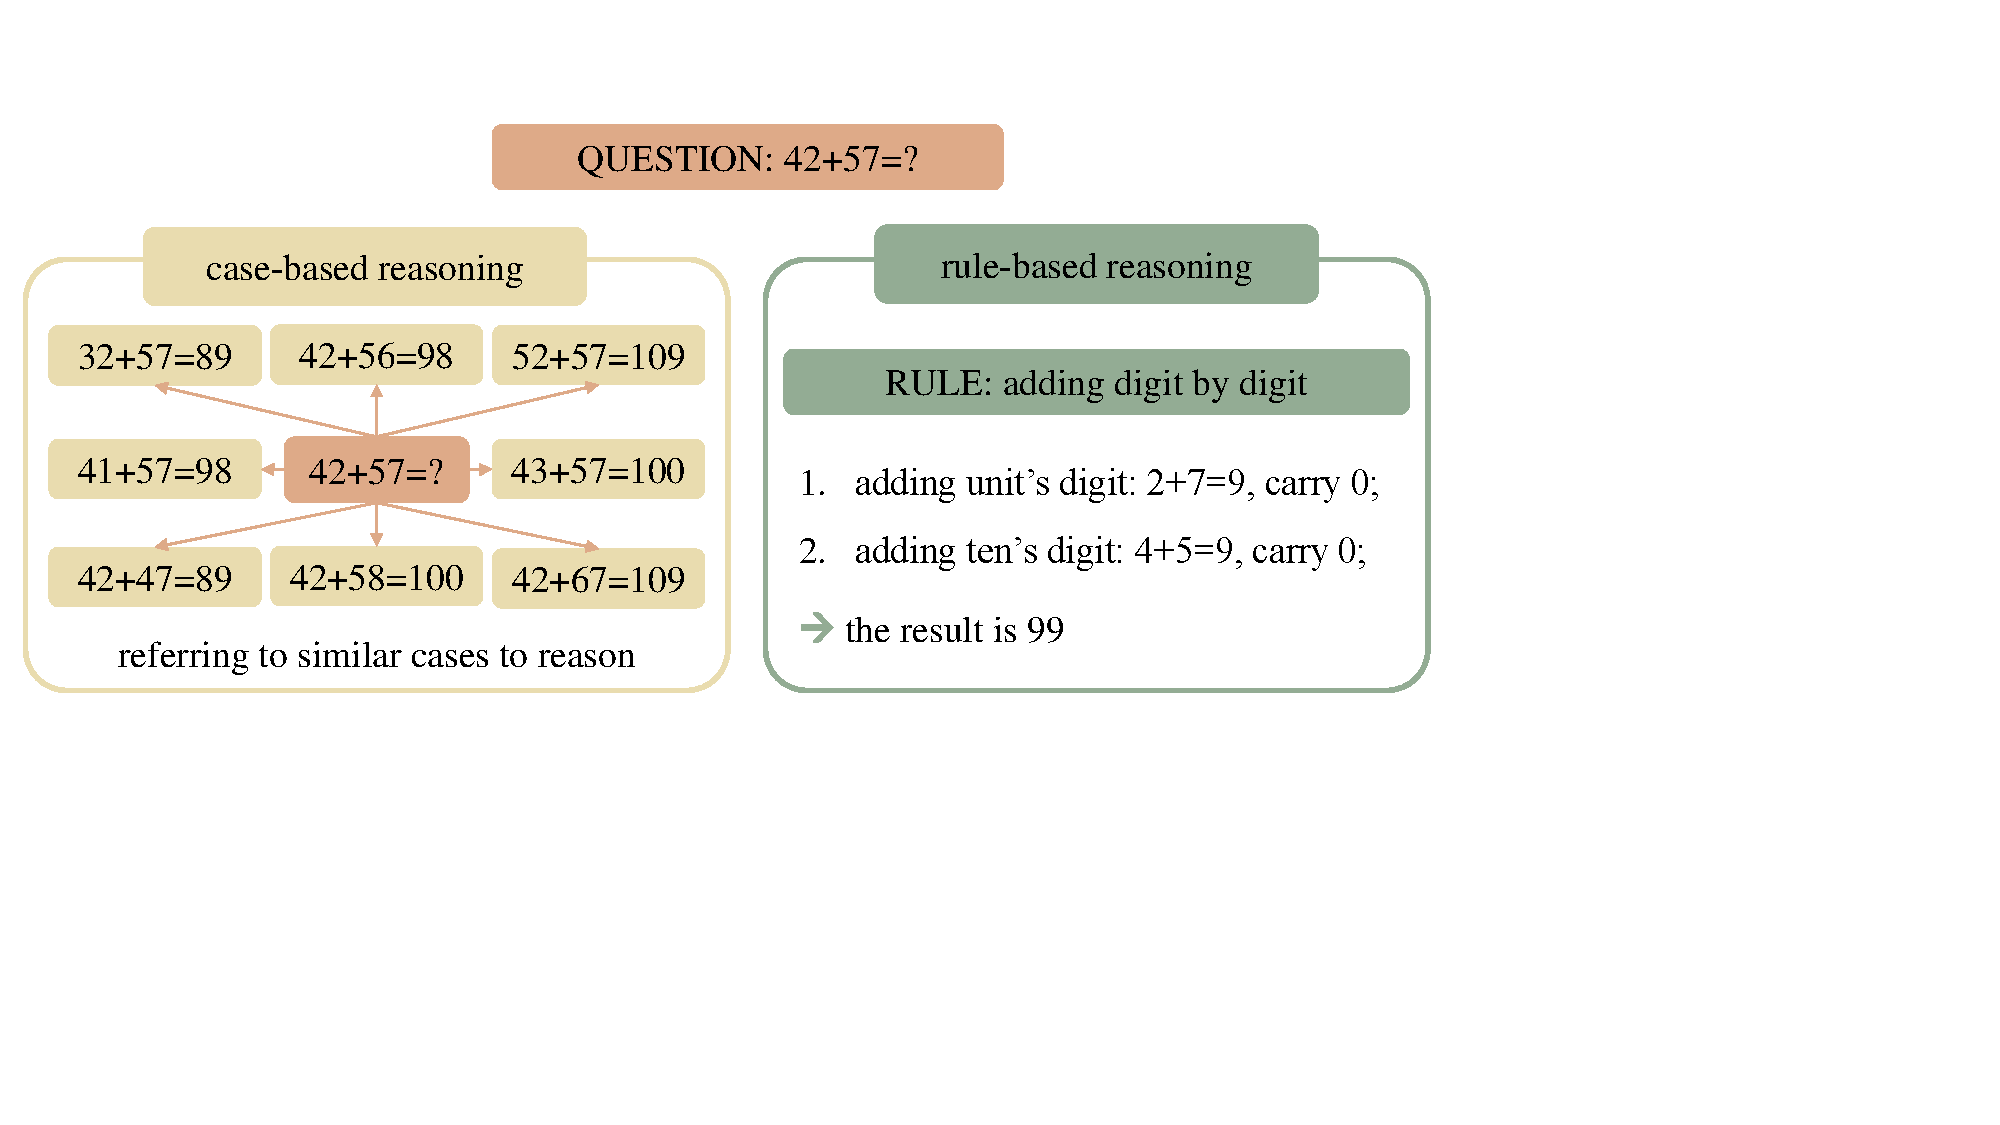
\includegraphics[width=\textwidth]{pic/case-or-rule.pdf}
					\caption{Illustrations of case-based and rule-based reasoning.}
					\label{case-or-rule}
				\end{figure}
			}
		\end{column}
		% \pause
		\begin{column}{0.2\textwidth}\onslide<3->{
				rule-based 依赖数学规则,即使语料库中没有这个问题,也可以根据从语料库中学习到的数学规则推理出正确的答案。}
		\end{column}
	\end{columns}
\end{frame}

\subsection{Leave-Square-Out method}
\begin{frame}{Leave-Square-Out method} \small
	% \begin{exampleblock}{什么是Leave-Square-Out method?}
	Leave-Square-Out method (留方法,LSO) 是作者提出的一种交叉验证(cross-validation)方法,用于评估机器学习模型的性能。它是留一法(Leave-One-Out)的扩展。与留一法相比,Leave-Square-Out 方法不是每次只留一个样本进行测试,而是每次留出 $k^2$ 个样本进行测试,其中 $k$ 是一个正整数。当数据集规模较大时,这种方法可以更好地评估模型的泛化能力。
	\pause
	% \end{exampleblock}
	\begin{figure}[t]
		\centering
		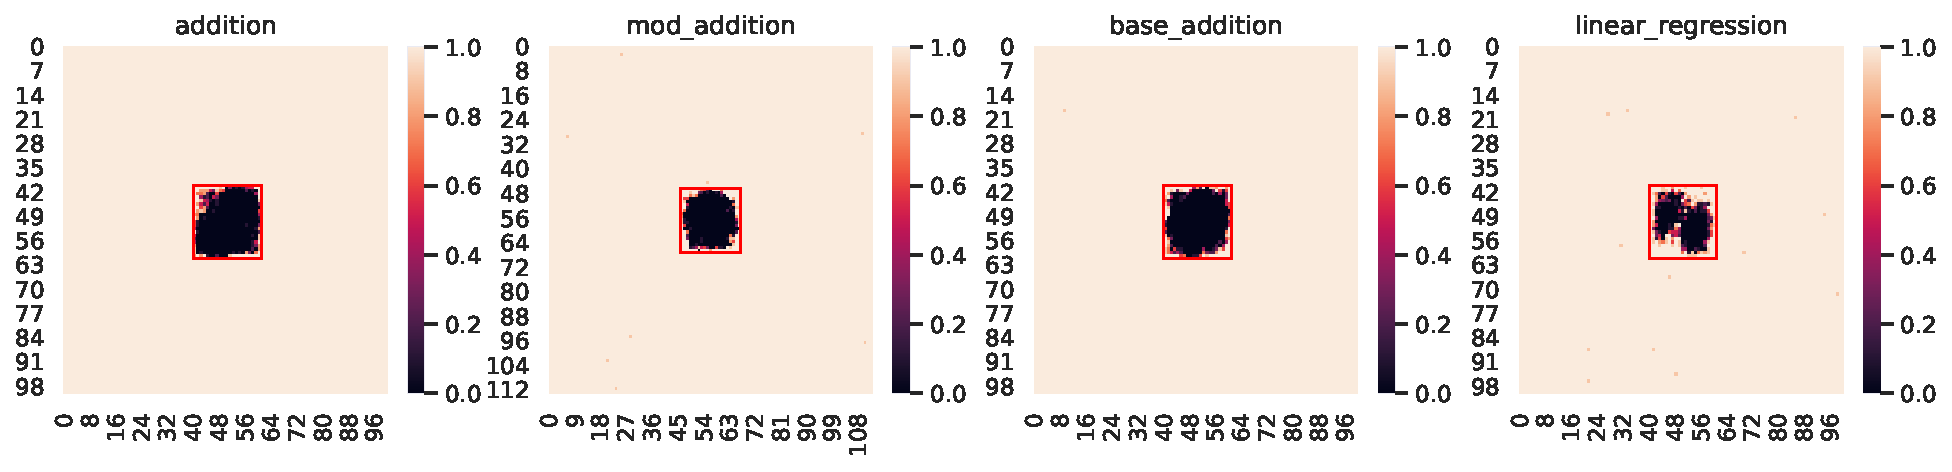
\includegraphics[height=0.3\textheight]{pic/1holes_w_rec_red_compressed.pdf}
		% \vspace{-10pt}
		\caption{Accuracy of Leave-Square-Out method}
		\label{fig:holes}
	\end{figure}
	\pause
	The appearance of holes in the figure indicates that the test samples away from the boundary of the training set are hard for the models to correctly infer.
\end{frame}

\subsection{rule-based setting}
\begin{frame}{rule-based setting}
	\begin{exampleblock}{rule based 的重要性}
		Rule-based reasoning is essential for models to achieve systematic and length generalization so that they can be applied to new, unseen scenarios without re-training.
	\end{exampleblock}
	\pause
	\begin{exampleblock}{rule based 应注意的事情}
		training set should always provide the necessities for the model to learn the underlying rule. For example, the training set should at least cover all the tokens used in the test set in order to develop a systematic rule that applies to the whole dataset.
	\end{exampleblock}

\end{frame}

\subsection{实验结论}
\begin{frame}{实验结论}
	\begin{itemize}
		\item test squares 的位置不会影响实验结果
		      \pause
		\item test squares 的大小会影响实验结果(the hole disappears when the test square shrinks to less than a small size)
		      \pause
		\item scratchpad cannot teach transformers to perform rule-based reasoning. (why? scratchpad fine-tuning fails to teach transformers the actually applied "rule" behind each step. This is like teaching children addition only by showing them examples, without telling them the rationales behind each step.)
		      \pause
		\item 模型和数据集的增大几乎不会影响实验结果,“holes”仍然存在
	\end{itemize}
\end{frame}

  \section{LLMs-based Methods}
\subsection{Instruction Learning}
\begin{frame}
	\frametitle{Instruction Building}
	\begin{small}
	Instruction Building 是利用 LLMs 创建数据集的阶段。\\ 
	WizardLM 使用了 Evol-Instruct 方法让 LLM 自动生成高质量的 Instructions.
	\end{small}
	\begin{columns}
		\begin{column}{.2\textwidth}
			Evol-Instruct 从广度、深度、增加约束条件、具象化等方面演化。
		\end{column}
		\begin{column}{.8\textwidth}
	\begin{figure}[h]
		% \vspace{-2mm}
		\begin{center}
			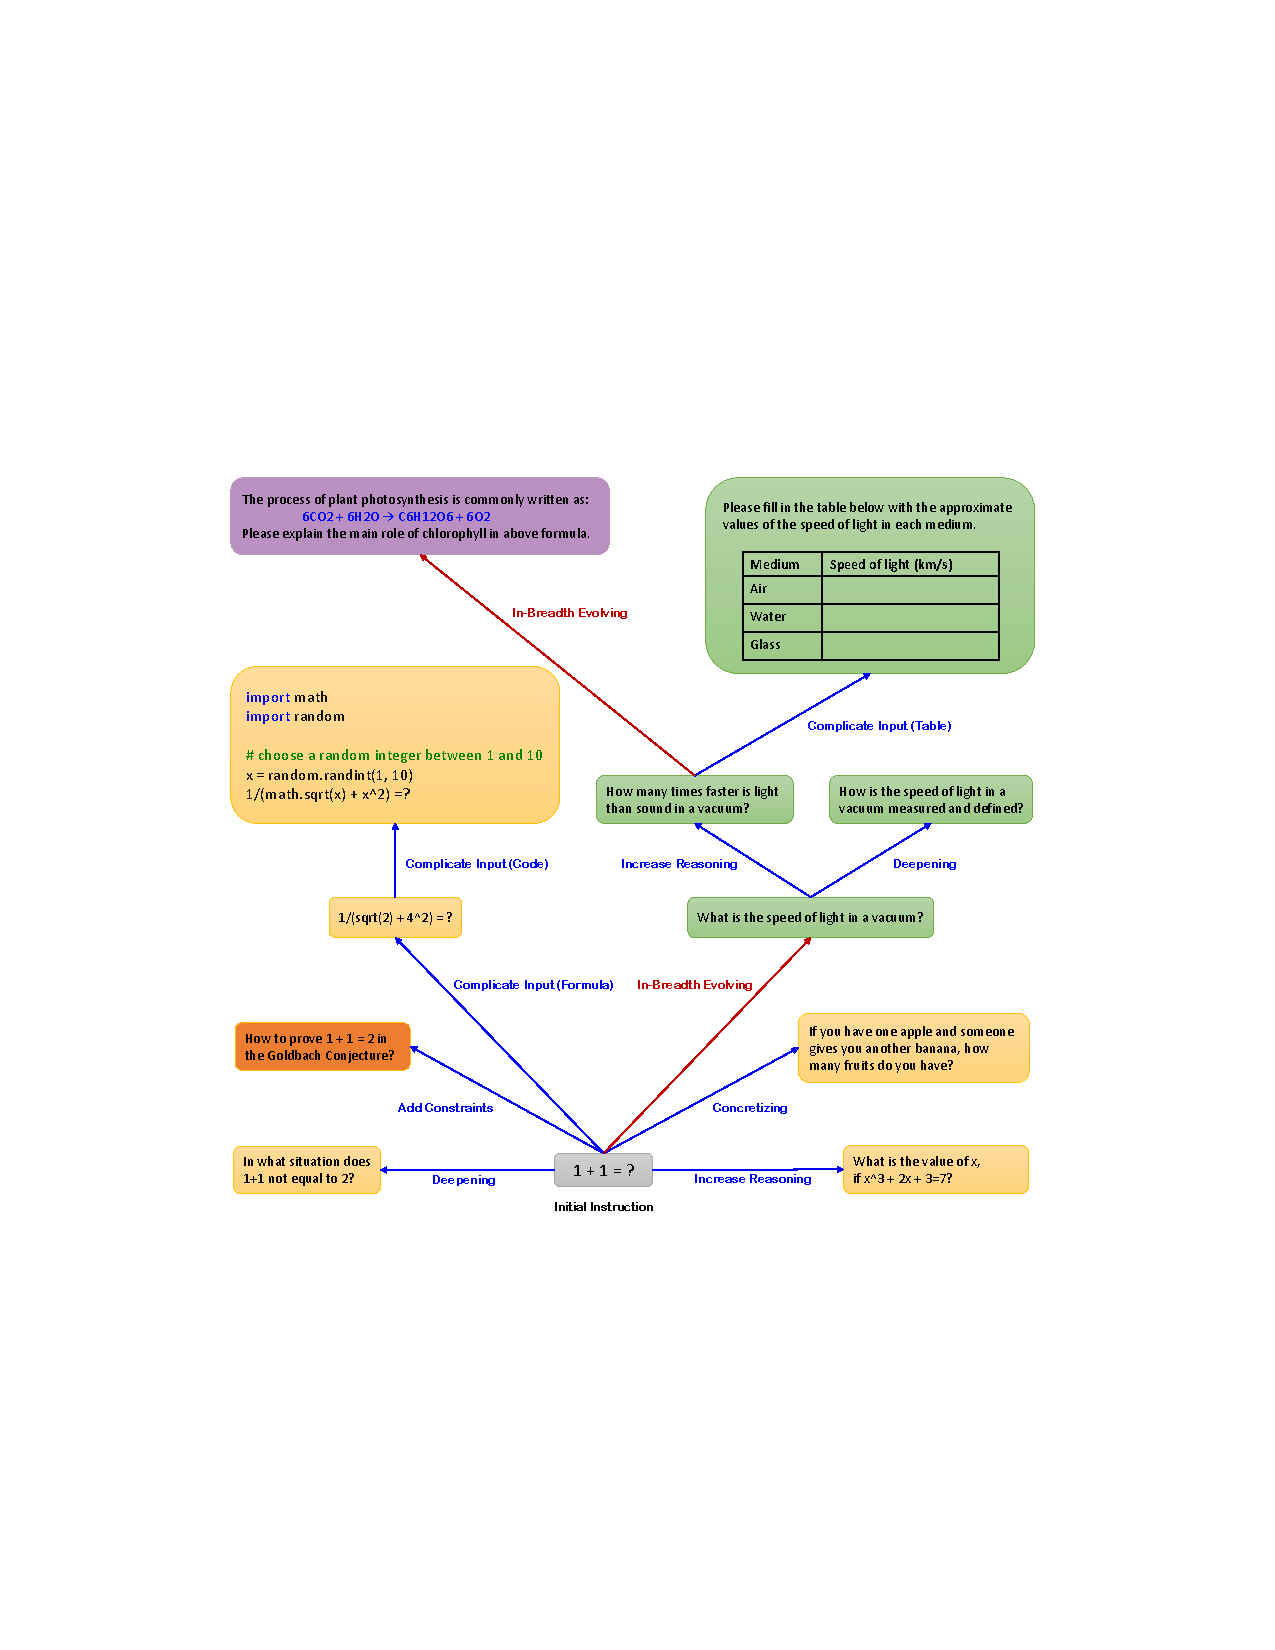
\includegraphics[width=0.5\textwidth]{pic/WizardLM.pdf}
		\end{center}
		\caption{Example of Evol-Instruct taken from WizardLM}
		\label{Evol-Instruct}
	\end{figure}
\end{column}
\end{columns}
\end{frame}

\begin{frame}
	\frametitle{Reinforcement Learning from Evol-Instruct
		Feedback (RLEIF)}
		\begin{columns}
			\begin{column}{.2\textwidth}
				{\small RLEIF 在 Evol-Instruct 的基础之上增加了  Process-supervised Reward Model (PRM) 作为监督模型,在 proximal policy optimization (PPO) 阶段会综合考虑这两个 reward model 的得分。}
			\end{column}
			\begin{column}{.8\textwidth}
	\begin{figure}
		\centering
		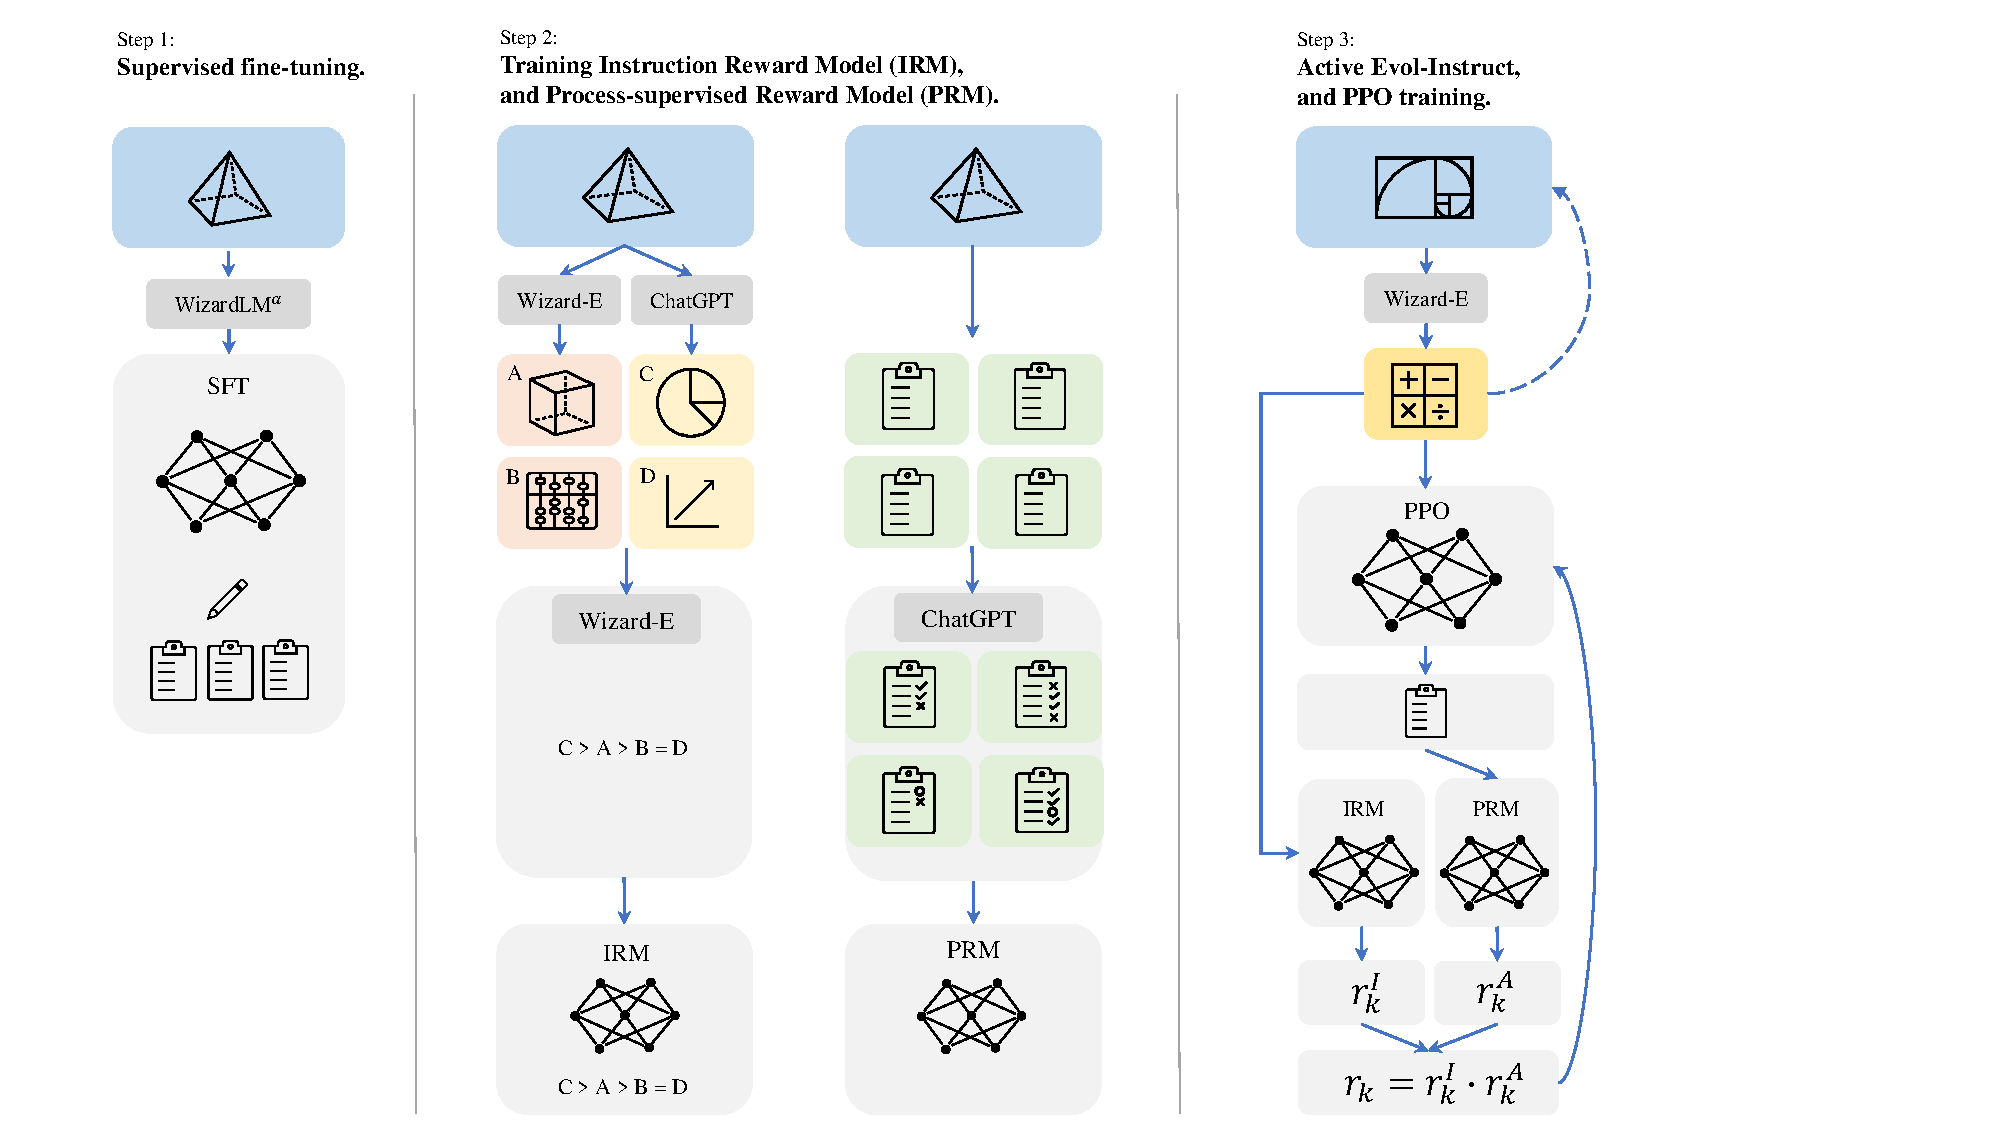
\includegraphics[width=0.7\textwidth, scale=1, trim=39 0 175 0,clip]{pic/reinforcement_evol_instruct.pdf}
		\caption{A diagram illustrating the three steps of RLEIF}
		\label{fig:reinforcement_evol_instruct_pic}
	\end{figure}
\end{column}
\end{columns}
\end{frame}

\begin{frame}
	\frametitle{Instruction Tuning}
	\textbf{PaLM 2-L-Math}:
	\begin{itemize}
		\item 发现 step-by-step 对于解题的质量提升有明显的效果。
		\item 综合使用 solution re-ranking 与 majority voting 会比单独使用效果更好。
		\item 通过多任务微调的方法,将生成解答和评估解答这两个任务分开,可以获得比只对解答进行单一微调更好的效果。
	\end{itemize}
\end{frame}

\begin{frame}
	\frametitle{In-context Learning (ICL)}
	ICL 是指通过在推理时提供特定任务示例,而无需更新模型参数。
	\begin{itemize}
		\item \textbf{ScratchpadGPT:}要求模型在 Scratchpad 中输出中间计算步骤,提升了正确率。
		\pause 
		\item \textbf{Codex-math:}通过生成代码的方式结合少样本学习自动生成解决数学问题的代码。
		\pause
		\item 选择复杂且多样化的示例可以提升推理性能。
	\end{itemize}
\end{frame}
  \section{安装运行}

\subsection{运行 Ollama}

\begin{frame}[fragile]
\frametitle{运行 Ollama}
\textbf{启动 Ollama 服务}
\begin{lstlisting}[language=bash]
export OLLAMA_MODELS=/usr/share/ollama/.ollama/models
export OLLAMA_HOST=0.0.0.0
export OLLAMA_SCHED_SPREAD=1
export CUDA_VISIBLE_DEVICES=0,1,2,3,4,5,6,7

nohup sh -c 'ollama serve' > ollama.log 2>&1 &
\end{lstlisting}
\begin{itemize}
    \item \textbf{注意}:
    \begin{itemize}
        \item \texttt{OLLAMA\_HOST} 必须设置为 \texttt{0.0.0.0},否则后续 Open Webui 无法访问 Ollama。
        \item \texttt{OLLAMA\_SCHED\_SPREAD} 必须设置为 \texttt{1},否则无法多卡运行单一模型。
    \end{itemize}
\end{itemize}
\end{frame}

\begin{frame}[fragile]
\frametitle{拉取 DeepSeek R1}
% \subsection{拉取 DeepSeek R1 模型}
\textbf{使用 Ollama 拉取 DeepSeek R1 模型}
\begin{lstlisting}[language=bash]
ollama pull deepseek-r1:671b # 默认就是 q4_K_M 量化
\end{lstlisting}
\end{frame}

\subsection{使用 Open Webui 对话}
\begin{frame}
\frametitle{使用 Open Webui 对话}
% \subsubsection{Open Webui 配置}
\textbf{Open Webui 后端地址设置}
\begin{figure}
    \centering
    
\includegraphics[width=\textwidth]{./pic/1.png} % 替换为你的图片路径
    % \caption{Open Webui 后端地址设置示例}
    \label{fig:openwebui_backend}
\end{figure}
% \textit{图片来源: \url{https://raw.githubusercontent.com/Lanthanum1/my_images/main/img/202502112050602.png}} % 图片来源注释
\end{frame}

\begin{frame}
\frametitle{Open Webui 配置详解}
% \subsubsection{Open Webui 配置详解}
\begin{itemize}
    \item Open Webui 配置分三层:模型级, 账户级, 聊天级。
    \item 优先级: 模型级 > 账户级 > 单次聊天级。
    \item \textbf{单次聊天级 (Per-Chat)}: 聊天右侧 Chat Controls 中设定,仅对当前会话生效,不能覆盖模型预设。
    \item \textbf{模型级 (Per-Model)}: Admin Panel-Settings-Models 中设定,适用于所有使用该模型的聊天,优先级最高。
    \item \textbf{账户级 (Per-Account)}: Settings-Advanced Parameters 中设定,会被模型级配置覆盖。
\end{itemize}
\end{frame}

\begin{frame}
\frametitle{Open Webui 调整参数}
% \subsubsection{Open Webui 性能调优}
\begin{itemize}
    \item 8 卡 A100 在设定Context Length和Max Tokens都为8k后可正常推理,每张卡显存占用约为50-60GB.
    \item 默认情况下,5min内如果没有新的对话,模型会从 GPU 中 offload,重新加载至显存需要很长时间。可以在 Settings-Advanced Parameters 中设定 Keep Alive 参数,设为 -1 则用不卸载。
    \item  如果显存不够,可通过设置 \texttt{num\_gpu} 参数来灵活调整 CPU/GPU 推理比例。
        \begin{itemize}
            \item 例如设为 \texttt{60} 则 60 层加载到 GPU,剩余在 CPU 推理。
        \end{itemize}
		\item 完成上述配置后,即可在 Open Webui 中与 DeepSeek R1 模型进行对话。
\end{itemize}
\end{frame}

% \begin{frame}
% \frametitle{Open Webui 对话}
% % \subsubsection{开始对话}
% \begin{itemize}
    
% \end{itemize}
% \end{frame}	
  %   \section{其他尝试}

\begin{frame}
    使用 Ollama 并不是最优选择,无论是速度还是显存占用都是不佳的。

    \texttt{OLLAMA\_SCHED\_SPREAD=1} 本来也是不建议开启的,Ollama 只能用单一的 gguf 格式的模型参数进行推理,但是对于 671 B 这么大的模型来说,全部加载在同一张 GPU 上是不太现实的,只能分担在多张GPU上,Ollama 对于一个模型在多卡中推理优化较差,这样做增加了GPU之间通信的成本,即使所有参数全部在GPU中推理,速度也只有 10-40 tokens/s。
\end{frame}

\begin{frame}
    \frametitle{vllm}
    \begin{itemize}
        \item \textbf{vllm}可能是比 Ollama 更优的选择。
              \begin{itemize}
                  \item 原生支持 safetensor 格式。
                  \item 但是 671B fp8 太大了,8卡a100也装不下。
              \end{itemize}

              \bigskip

        \item 考虑使用量化模型以降低显存需求。
              \begin{itemize}
                  \item vllm官网中有一句话,Please note that GGUF support in vLLM is highly experimental and under-optimized at the moment, it might be incompatible with other features.
                  \item 尝试 1.58 bit 动态量化版本报错 (ValueError: GGUF model with architecture deepseek2 is not supported yet.)。
                  \item INT4 W4A16 量化可能是可行的方案 (未尝试)。
              \end{itemize}
    \end{itemize}
\end{frame}

\begin{frame}[fragile]
    \frametitle{模型下载问题}
    \subsubsection{模型下载问题}
    \begin{itemize}
        \item 拉取 1.58 bit 动态量化模型时,\texttt{hf mirror} 速度慢且易断连。
        \item \texttt{modelscope} 限速在 15MB/s 左右。
        \item 对于 671B 这么大的模型,可以使用 \texttt{snapshot\_download} 下载部分文件夹。
    \end{itemize}
    % \textbf{使用 \texttt{snapshot\_download} 下载部分文件夹示例 }
    \begin{lstlisting}[language=python]
from huggingface_hub import snapshot_download
snapshot_download(repo_id='unsloth/DeepSeek-R1-GGUF', allow_patterns='DeepSeek-R1-UD-IQ1_S/*', cache_dir='./')

# modelscope

from modelscope.hub.snapshot_download import snapshot_download
model_dir = snapshot_download(repo_id='unsloth/DeepSeek-R1-GGUF', allow_patterns='DeepSeek-R1-UD-IQ1_S/*',cache_dir='./')
\end{lstlisting}
\end{frame}

\fi


\end{document}

